\chapter{Layered Editor Architectures}
\label{chap:layeredArchs}
{\em *** Version: \today~ ***}


\bc

IMPORTANT there seems to be an invariant that for a j:  i>j, all mappings are correct 
  ..           ...       
 .  .    ..   .   .   .. 
.    ....  ...     ...  .
no it's not asymmetric. find out more about this.
maybe it's just that a level is never presented twice without intr, and vice versa


MAYBE DO SOME NON layered stuff first? to explain what spec. will mean. more important if things like intention of edit op is added as an equation.
\ec


% intro

\bc
Using the single layer specification from the previous chapter, we can give a specification for a layered editor architecture. The building blocks for the specification are . The specification for a single layer from the previous chapterprev. chap. spec for layer but not edit and transform. Edit result in new lower level, initiated by gesture from user. Transform higher. In this chapter,level take all layers together and combine. At top and bottom, some extra stuff.
\ec
\bl
\o Spec for editor is combined spec for single layers.
\o abstract $Edit$ and $Transform$ removed
\o Next chapter, we give Haskell for the combination.
\el


\bl
\o In this chapter, combine the single layer specifications.
\o First combine everything, assuming edit ops are indirect (ref Chapter Edit Model)
\o Section~\ref{sect:specHigherEdit} support for direct interpretation of edit ops
\o Section~\ref{sect:specSkipLayers} support for skipping higher layers
\el
\fromHere  % VVVVVVVVVVVVVVVVVVVVVVVVVVVVVVVVVVVVVVVVVVVV

\section{Specifying a layered editor}\label{sect:specCombination}

The basic component for combining the layers is the incremental specification of a single layer, given in Section~\ref{sect:maintainingInc} of the previous chapter. The specification of a layered editor consists of a combination of several instances of the single layer specification. Before we combine the specifications, we first construct a diagram that sketches the combination process.


\subsection{Combining layers in a diagram}
\note{Add arrow stating that the result is what we mean with the gesture? (eg. $level''_n = Intended~e_n~level_n~(\dots level_0)$)}

\bc The lefthand side of \ec Figure~\ref{singleToMulti1} shows a simplified version of the final diagram (Figure~\ref{maintainExtraState}) from Section~\ref{sect:maintainingInc}. Except for the level updates, all internal data flow is hidden, showing only the input and output values of the level. The updates are not hidden, because some updates need to be removed for the combination.\note{first explain non-layered situation? Or is this clear enough?}




\bc
\begin{figure}\begin{small}\begin{center}\begin{center}
\epsfig{file=pics/eps/singleToMulti.eps, width=125mm}\end{center}
\caption{A single layer vs. Layer $i$.}\label{singleToMulti} 
\end{center}\end{small}\end{figure}\note{split this figure in two figures next to each other?}
\ec
\begin{figure}[h]
  \hfill
  \begin{minipage}[b]{.45\textwidth}
    \begin{center}  
      \epsfig{file=pics/eps/singleToMulti1.eps, width = 60mm}
      \caption{A single layer.} \label{singleToMulti1}
    \end{center}
  \end{minipage}
  \hfill
  \begin{minipage}[b]{.45\textwidth}
    \begin{center}  
      \epsfig{file=pics/eps/singleToMulti2.eps, width = 60mm}
      \hfill
      \caption{$Layer_i$.} \label{singleToMulti2}
    \end{center}
  \end{minipage}
  \hfill
\end{figure}

To be able to combine the layer, the $H$ and $L$ subscripts are replaced by indices. Because the document is $level_0$, and the rendering is $level_n$, a higher level gets an index $i$ whereas a lower level gets an index $i+1$. The functions ${\tt interpret}$ and ${\tt present}$ get a subscript $i$. \bc The righthand side of \ec Figure~\ref{singleToMulti2} contains the resulting indexed layer. Note that the abstract functions $Edit$ and $Transform$ have been dropped because adjacent layers will now take care of this functionality.

The layer in Figure~\ref{singleToMulti2} cannot be combined yet, because on interpretation and presentation, it updates both the upper level ($i$) and the lower level ($i+1$). Thus, we drop one update in the interpration phase and one in the presentation phase. Section~\ref{sect:incrementalSpec} explained that an implementation of a mapping function may perform an update on the source level of the mapping (ie. 
${\tt interpret}$ may update the lower level, and ${\tt present}$ may update the higher level). In order to still allow this behavior, we drop the updates on the target levels: the higher level update in the interpretation phase (upper left dotted arrow), and the lower level update in the presentation phase (lower right dotted arrow). 

\bc The lefthand side of \ec Figure~\ref{combiningLayers1} shows a layer without the two target level updates. When several layers are combined, we get the diagram in Figure~\ref{combiningLayers2}.

\bc
\begin{figure}\begin{small}\begin{center}\begin{center}
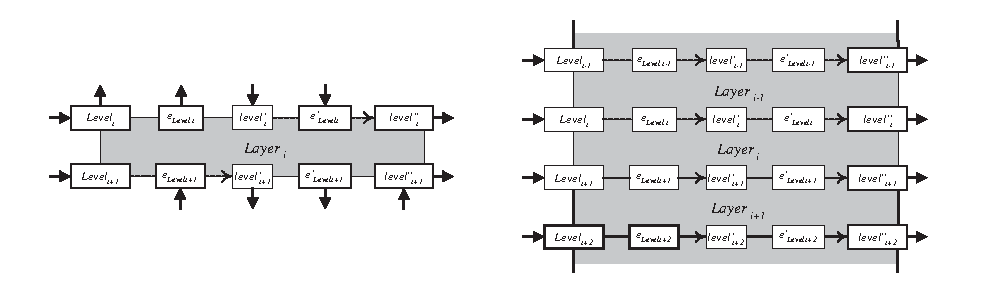
\epsfig{file=pics/eps/connectingLayers.eps, width=125mm}\end{center}
\caption{A layer with only two updates vs Combined layers}\label{combiningLayers} 
\end{center}\end{small}\end{figure}
\ec

\begin{figure}[h]
  \hfill
  \begin{minipage}[b]{.45\textwidth}
    \begin{center}  
      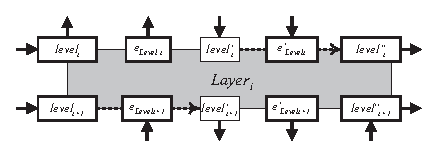
\epsfig{file=pics/eps/connectingLayers1.eps, width = 60mm}
      \caption{Layer $i$ with two updates.} \label{combiningLayers1}
    \end{center}
  \end{minipage}
  \hfill
  \begin{minipage}[b]{.45\textwidth}
    \begin{center}  
      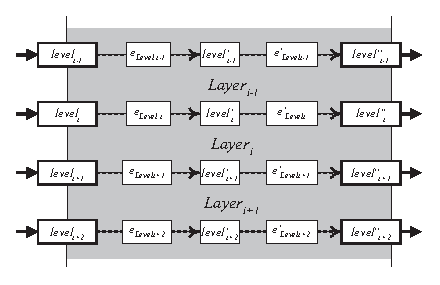
\epsfig{file=pics/eps/connectingLayers2.eps, width = 60mm}
      \caption{Combined layers.} \label{combiningLayers2}
    \end{center}
  \end{minipage}
  \hfill
\end{figure}


The combination in Figure~\ref{combiningLayers2}, shows what happens for internal layers that are surrounded by other layers. However at the top and the bottom of the layered architecture, still some work needs to be done. At the top, edit operations coming out of the interpretation phase need to be put back into the presentation phase. And at the bottom, an edit gesture from the user must be put into the combined layers combination, and an updated rendering must be shown to the user. The lefthand side of Figure~\ref{topAndBottom} shows the loose ends that need to be dealt with.

\begin{figure}\begin{center}\begin{center}
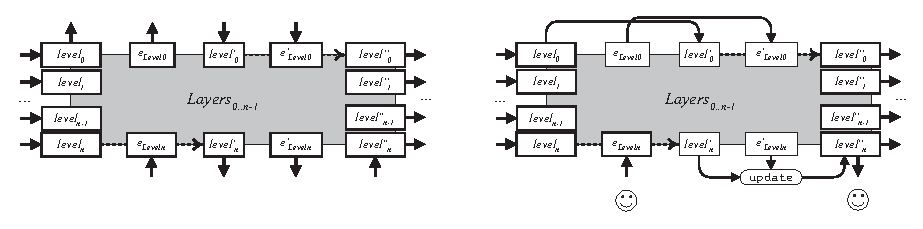
\epsfig{file=pics/eps/topAndBottom.eps, width=125mm}\end{center}
\caption{Loose ends at the top and bottom vs Dataflow at the top and bottom}\label{topAndBottom} 
\end{center}\end{figure}

\note{gesture depends on level, not edit. Also on other levels?}

At the top, the result of the combined interpret mappings is a document edit operation $e_{Level_0}$. Because the target update of each layer has been dropped, the operation is not performed on the document $level_0$. Rather than explicitly adding an update, we put the level and the edit operation back into the presentation part of the combined layers. This way, the document update is performed by the presentation phase of the top layer.

Similar to situation at the top, the bottom of the layer combination also misses an update. Therefore, we add an update at the bottom right, which applies $e'_{Level_n}$ to $level'_n$. Furthermore, the edit gesture from the user needs to be fed into the layer structure, and the updated lower level needs to be shown to the user. The righthand side of Figure~\ref{topAndBottom} shows the data flow at the top and the bottom of the layers.

\subsection{Specifying combined layers}

We construct the specification of the combined layers along the same lines as the diagrams in the previous section. Recall that the data level definitions from a multiple layer perspective (see Section~\ref{sect:mappingInformation}) are:

\begin{small}\( \begin{array}{lcl}  \label{inv:incrementality}
\text{\bf type}~Level_{0}  =  Core_{Intr,0} \times Extra_{Intr,0} \times Info\idwn_{0} \\
\text{\bf type}~Level_{n}  =  Core_{Pres,n} \times Extra_{Pres,n} \times  Info\iup_{n}\\
\lefteqn{\forall j:1 \le i \le n-1:}  \\
\text{\bf type}~Level_{j} =  Core_{Pres,j} \times Extra_{Pres,j}  \times Info\iup_{j}   
                                       =  Core_{Intr,j} \times Extra_{Intr,j} \times Info\idwn_{j}
\end{array}\)\end{small}

First, we take the  final single layer specification from Section~\ref{sect:maintainingInc}, and replace the $H$ and $L$ subscripts by $i$ and $i+1$. Except for ${\tt update}$, the values and functions without an $H$ or $L$ subscript in specification~\ref{spec:incrementality} (${\tt sheet}$, ${\tt interpret}$, ${\tt present}$, and
 ${\tt reuse}$) are now specific to a certain layer and get an $i$ subscript. Because $update$ is a generic function it can be used in all layers without a subscript. Finally, we drop the equations for $Edit$ and $Transform$.

\begin{small}
\refstepcounter{specification} \label{spec:combinationFirstAttempt}
\( \begin{array}{lcl}
{\tt interpret_i}  ::  Sheet_{Intr,i} \rightarrow Level_{i+1} \rightarrow Level_{i} \rightarrow  Edit_{Level_{i+1}} \rightarrow Edit_{Core_{i}\times Info\idwn_{i}} \\
{\tt present_i}  ::  Sheet_{Pres,i} \rightarrow Level_{i} \rightarrow Level_{i+1}  \rightarrow Edit_{Level_{i}} \rightarrow Edit_{Core_{i+1}\times Info\iup_{i+1}}\\
\\
\end{array}\) \\
\( \begin{array}{rcll}  
level_{i+1} 	& = & Present_{i}~level_{i}						& \text{\{Precondition\}}\\
\\
level'_{i+1} 	& = & {\tt update}~e_{Level_{i+1}}~level_{i+1}                 & \text{\{Compute intermediate lower level\}}\\
e_{Core_{i} \times Info\idwn_{i}}  & = & {\tt interpret}_{i}~sheet_{Intr,i}~level_{i+1}~level_{i}~e_{Level_{i+1}} & \text{\{Compute higher core update\}}\\
e_{Level_{i}} & = & {\tt reuse}_{Intr,i}~level_{i}~e_{Core_{i}\times Info\idwn_{i}}     & \text{\{Reuse extra state\}}\\
level'_{i} & = & {\tt update}~e_{Level_{i}}~level_{i}                 & \text{\{Compute intermediate higher level\}}\\
\\\
level'_{i} & = & Interpret_{i}~level'_{i+1}						& \text{\{Intermediate condition\}}\\
\\
level''_{i} & = & {\tt update}~e'_{Level_{i}}~level'_{i}                 & \text{\{Compute final higher level\}}\\
e'_{Core_{i+1}\times Info\iup_{i+1}}  & = & {\tt present}_{i}~sheet_{Pres,i}~level'_{i}~level'_{i+1}~e'{Level_{i}} & \text{\{Compute new lower core\}}\\
e'_{Level_{i+1}} & = & {\tt reuse}_{Pres,i}~level_{i+1}~e'_{Core_{i+1}\times Info\iup_{i+1}} & \text{\{Reuse extra state\}}\\
level''_{i+1} & = & {\tt update}~e_{Level_{i+1}}~level_{i+1}                 & \text{\{Compute final lower level\}}\\
\\
level''_{i+1} & = & Present_{i}~level''_{i}						& \text{\{Postcondition\}}\\
\end{array}\)
\end{small}
\begin{center}(Specification \thespecification: First attempt)\end{center}\vspace{1em}

\note{what to do about levels and layers subscript mismatch layers 0..n-1 levels 0..n?}

The specification does not yet define $e_n$ and $e'_0$, and similar to the diagrams of the previous section it has double updates on all levels but the document and the rendering. This is because updates for ${\tt level}$ and ${\tt level'}$ are specified on the higher level $i$ as well as the lower level $i+1$. We solve the problem in the same way as in the previous section, by dropping the updates on the target levels (equations \{Compute intermediate higher level\} and \{Compute final lower level\}). The remaining updates are:

\begin{small}\( \begin{array}{lcll} 
level'_{i+1} 	& = & {\tt update}~e_{Level_{i+1}}~level_{i+1}                 & \text{\{Compute intermediate lower level\}}\\
level''_{i} & = & {\tt update}~e'_{Level_{i}}~level'_{i}                 & \text{\{Compute final higher level\}}\\
\end{array}\)
\end{small}

Because of the dropped updates, there are no computations for $level'_0$ and $level''{n}$. And moreover, $e_n$ and $e'_0$ need to be defined. At the top, the document and the edit operation on it ($level_0$ and $e_0$) are put back into the computation by assigning them to $level'_0$ and $e'_0$, yielding:

\begin{small}\( \begin{array}{lcll} 
e'_{Level_{0}}  = e_{Level{0}}\\
level'_{0} =  level_{0}\\
\end{array}\)
\end{small}

At the bottom, we add a rendering update on $level'_n$ and specify that $e_n$ is the edit gesture that comes from the user. The fact that the updated rendering $level''_n$ is shown to the user is not explicitly visible in the specification.

\begin{small}\( \begin{array}{lcll} 
e_{Level_{n}}  = EditGesture ??\\
level''_{n}  =  {\tt update}~e'_{Level_{n}}~level'_{n}\\
\end{array}\)
\end{small}

If we remove the double updates and add the equations for handling the top and bottom cases, we get the final specification:

\begin{small}
\refstepcounter{specification} \label{spec:combination}
\( \begin{array}{lcl} 
\text{\bf type}~Level_{0}  =  Core_{Intr,0} \times Extra_{Intr,0} \times Info\idwn_{0} \\
\text{\bf type}~Level_{n}  =  Core_{Pres,n} \times Extra_{Pres,n} \times  Info\iup_{n}\\
\lefteqn{\forall j:1 \le i \le n-1:}  \\
\text{\bf type}~Level_{j} =  Core_{Pres,j} \times Extra_{Pres,j}  \times Info\iup_{j}   
                                       =  Core_{Intr,j} \times Extra_{Intr,j} \times Info\idwn_{j}\\
e_{Level_{n}}  = EditGesture ??\\
e'_{Level_{0}}  = e_{Level{0}}\\
level'_{0} =  level_{0}\\
level''_{n}  =  {\tt update}~e'_{Level_{n}}~level'_{n}\\
\lefteqn{\forall i:0 \le i \le n-1:}  \\
{\tt interpret_i}  ::  Sheet_{Intr,i} \rightarrow Level_{i+1} \rightarrow Level_{i} \rightarrow  Edit_{Level_{i+1}} \rightarrow Edit_{Core_{i}\times Info\idwn_{i}} \\
{\tt present_i}  ::  Sheet_{Pres,i} \rightarrow Level_{i} \rightarrow Level_{i+1}  \rightarrow Edit_{Level_{i}} \rightarrow Edit_{Core_{i+1}\times Info\iup_{i+1}}\\
\\
\end{array}\) \\
\( \begin{array}{rcll}  
level_{i+1} 	& = & Present_{i}~level_{i}						& \text{\{Precondition\}}\\
\\
level'_{i+1} 	& = & {\tt update}~e_{Level_{i+1}}~level_{i+1}                 & \text{\{Compute intermediate lower level\}}\\
e_{Core_{i} \times Info\idwn_{i}}  & = & {\tt interpret}_{i}~sheet_{Intr,i}~level_{i+1}~level_{i}~e_{Level_{i+1}} & \text{\{Compute higher core update\}}\\
e_{Level_{i}} & = & {\tt reuse}_{Intr,i}~level_{i}~e_{Core_{i}\times Info\idwn_{i}}     & \text{\{Reuse extra state\}}\\
\\\
level'_{i} & = & Interpret_{i}~level'_{i+1}						& \text{\{Intermediate condition\}}\\
\\
level''_{i} & = & {\tt update}~e'_{Level_{i}}~level'_{i}                 & \text{\{Compute final higher level\}}\\
e'_{Core_{i+1}\times Info\iup_{i+1}}  & = & {\tt present}_{i}~sheet_{Pres,i}~level'_{i}~level'_{i+1}~e'{Level_{i}} & \text{\{Compute new lower core\}}\\
e'_{Level_{i+1}} & = & {\tt reuse}_{Pres,i}~level_{i+1}~e'_{Core_{i+1}\times Info\iup_{i+1}} & \text{\{Reuse extra state\}}\\
\\
level''_{i+1} & = & Present_{i}~level''_{i}						& \text{\{Postcondition\}}\\
\end{array}\)
\end{small}
\begin{center}(Specification \thespecification: Final specification)\end{center}\vspace{1em}

The specification describes the behavior of the editor for a single edit step. The state of the editor is formed by all data levels together. At the start of an edit step, the $Presentation$ invariant holds an each layer. 

Given an initial state ($level_{0\dots n}$) and an edit gesture from a user, the specification describes what needs to be computed in order to yield the state of the editor after the edit gesture is applied 
($level''_{0\dots n}$). The new state is the starting state for the next edit step.

When the editor application is started, each level gets an initial empty value . The levels are then updated  according to the specification, 
\toHere     % ^^^^^^^^^^^^^^^^^^^^^^^^^^^^^^^^^^^^^


Little story about what the invariant says:

Given $level_{0\dots n}$ for which Pres holds and an edit gesture, compute ($level''_{0\dots n}$) so Pres holds again.

\bl
\o level'' is level for next edit step
\o Starting the editor?
\o level for first needs to be initialized: empty vals, Present needs to hold
\o maybe first interpret is initializer, or load operation
\el


%																
%																
%																
\section{Edit operations  on higher levels} \label{sect:specHigherEdit}

\bl
\o assumed indirect. But edit on rendering and interpreting is not true (ref chapter arch) \note{Problem with direct/indirect terminology}
\o indirect and direct. Direct until layout level, and sometimes on enr. or doc.
\o need to fix
\o consequences for es safety
\o lower are not just skips, but direct edit op interpretations.
\o tricky. maybe need to point out diff between skipping and processing
\o kind of phase shift. Entire translation/presentation process is completed, but it starts at higher translation and also ends there.
\el

Spec:
\bl
\o edit op on level $j$ (== higher level for layer $j$)
\o $\forall i\le j:$ original spec. holds
\o $\forall i>j: e_j = skip$ 
\o $level'_j = Translate_j~level'_{j+1}$ does not hold $level''_{j+1} = Present_j~level''_j$ does
\o After edit op, need to translate at layers $n\dots j$ for mapping info.
\el 
\section{Skipping higher layers} \label{sect:specSkipLayers}
\bl
\o ref to edit model chapter
\o kind of optimization. 
\o skipping cycles + es safety
\o with update on only lower ES, automatic skip, but then no problem with invariants
\el

Spec:
\bl
\o skipping layers $0\dots j$
\o $\forall i>j:$ original spec. holds
\o $\forall i\le j: e_j and e'_j = skip and e'_{j+1} = e{j+1}$  
\o Invs. still hold, except at skipping point: $Translate_j$ and $Present_j$ do not hold.
\el

\section{Conclusions}

\bl
\o ?
\el




